\documentclass[12pt]{article}
\usepackage[utf8]{inputenc}
%\usepackage[portuguese]{babel}
\usepackage{amsmath,amsfonts,amssymb}
\usepackage{graphicx}
\usepackage{makeidx}
\usepackage{graphicx}
\usepackage{lmodern}
\usepackage{multicol}
\usepackage{booktabs}
\usepackage{fancyhdr}
\usepackage{hyperref}
\usepackage[usenames]{color}


\usepackage{Sweave}
\begin{document}
\Sconcordance{concordance:PCA-SVM.tex:PCA-SVM.Rnw:%
1 15 1 1 0 40 1 1 2 1 0 3 1 1 2 5 1 1 3 1 0 1 1 1 2 4 0 1 2 6 1 1 2 4 0 %
1 2 2 1 1 2 1 0 6 1 1 9 11 0 1 2 5 1 1 2 1 0 2 1 1 13 15 0 1 2 1 1 1 2 %
17 0 1 2 2 1 1 2 7 0 1 2 2 1 1 2 7 0 1 2 16 1}

\pagestyle{fancy}
\fancyhf{}
\renewcommand{\headrulewidth}{0.4pt}
\fancyfoot[C]{\thepage}
\renewcommand{\footrulewidth}{0.4pt}
\fancyfoot[C]{\thepage}
\title{\LARGE \bf
 Exercício  11 - PCA - SVM}
\author{ Rodrigo Machado Fonseca - 2017002253}
\thispagestyle{fancy}
\fancyhead[C]{Introdução ao Reconhecimento de Padrões - UFMG \\ Belo Horizonte - \today}
\maketitle
\thispagestyle{fancy}

%%%%%%%%%%%%%%%%%%%%%%%%%%%%%%%%%%%%%%%%%%%%%%%%%%%%%%%%%%%%%%%%%%%%%%%%%%%%%%%%%%%%%%%%%
\section{Introdução}

  \par Neste será implementado do método de Análise de Componentes Principais (PCA) e de uma Máquina de Vetores de Suporte (SVM) para realizar a classificação do conjunto de dados Breast Cancer.
  
\section{PCA}
  
  \par A técnica de PCA baseia-se em  reduzir a dimensionalidade de um conjunto de dados, preservando o máximo de “variabilidade” (ou seja, informações estatísticas) possível. Diminuir a dimensionalidade implica reduzir a complexidade do sistema, o que acarreta, menos gasto computacional para resolver determinados problemas. Além disso, reduzir a dimensionalidade implica a possibilidade de uma análise visual, o que não seria possível em um espaço de alta dimensão. 
  
  \par O algoritmo do PCA baseia-se nos seguintes passos:
  
  \begin{itemize}
    \item Calcula a média dos dados
    \item Subtrai a média dos dados 
    \item Calcula a matriz de covariância
    \item Encontre os auto-valores e auto-vetores
    
  \end{itemize}
  
\section{Experimento}

 \par A priori, será carregado a base \textit{Breast Cancer} e nela será aplicado o método PCA. Abaixo segue a figura da variância das componentes ordenadas:

\begin{figure}
\centering
\begin{Schunk}
\begin{Sinput}
> rm(list = ls())
> library(mlbench)
> library(caret)
> library('kernlab')
> data(BreastCancer) 
> db <- na.omit(BreastCancer) 
> db$Label[db$Class == "benign"] <- -1
> db$Label[db$Class == "malignant"] <- 1
> x <- data.matrix(db[,2:10])
> y <- data.matrix(db[,12])
> # PCA
> trans <- prcomp(x)
> PC <- predict(trans, x)
> screeplot(trans, type = "l", npcs = 9, main = "Variâncias das componentes ordenadas")
\end{Sinput}
\end{Schunk}
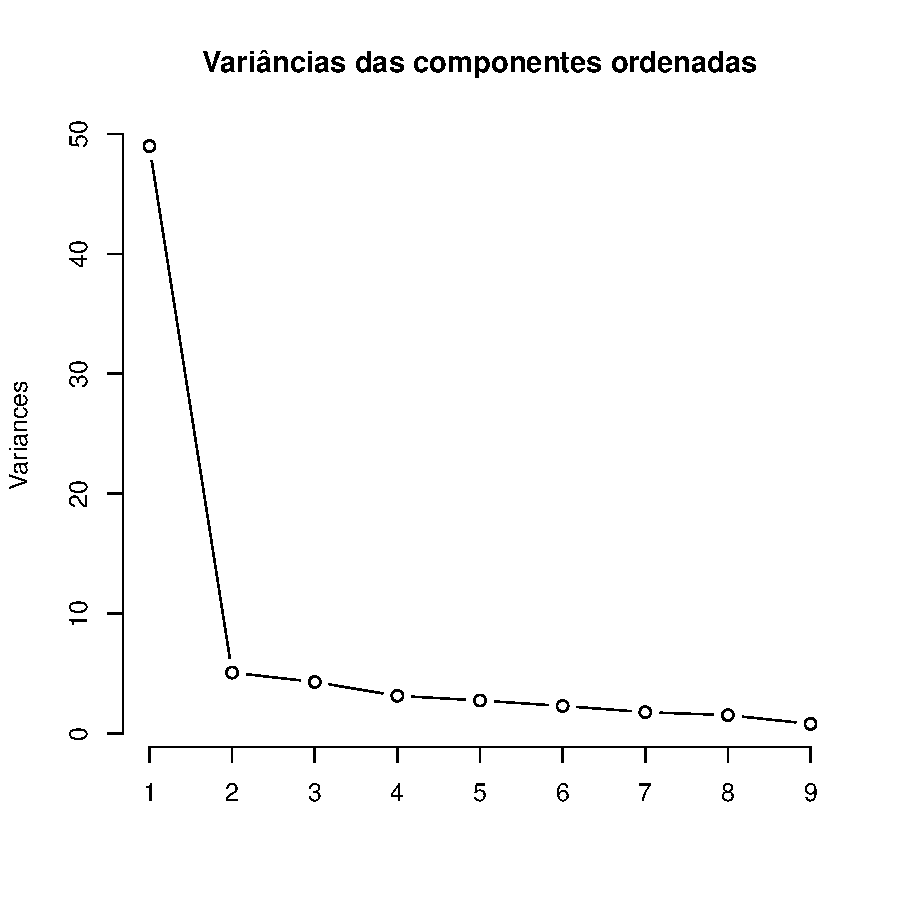
\includegraphics{PCA-SVM-001}
\caption{Gráfico da variância das componentes ordenadas}
\label{1}
\end{figure} 

  \par Em sequência, iremos definir o conjunto x de treinamento. 
  

\begin{Schunk}
\begin{Sinput}
> x <- PC[, 1:2]
\end{Sinput}
\end{Schunk}

\par  Por fim, separaremos o conjunto de dados  em 10 \textit{folds} para fazermos o treinamento. 
  
\begin{Schunk}
\begin{Sinput}
> set.seed(123)
> index <- sample(1:nrow(x), length(1:nrow(x)))
> step <- length(index) %/% 10
> step_vec <- seq(step, step*10, step)
> step_vec[10] <- length(index)
> flds <- list()
> j = 1
> for(i in step_vec){
+   if(j != 10){
+     flds[[j]] <- index[(i-67):i]
+   }
+   else{
+     flds[[j]] <- index[step_vec[j-1]:i]
+   }
+   j <- j+1
+ }
\end{Sinput}
\end{Schunk}
  

\section{Resultados}

  \par A seguir, está o treinamento para cada fold criado. 

\begin{Schunk}
\begin{Sinput}
> j = 1
> accuracy <- matrix(nrow = 10, ncol = 1)
> accuracy_fold <- matrix(nrow = 10, ncol = 2)
> for(i in flds){
+   x_train <- x[-i,]
+   y_train <- y[-i, ]
+   x_test <- x[i,]
+   y_test <- y[i, ]
+   svm <- ksvm(x_train,y_train,type='C-bsvc',kernel='rbfdot',kpar=list(sigma=0.5),C=1000)
+   y_hat <- predict(svm, x_test)*1
+   accuracy[j] <- sum((y_hat == y_test)*1)/length(y_hat)
+   
+   accuracy_fold[j, 1] <- sum((y_hat[y_hat==-1] == y_test[y_hat==-1])*1)/length(y_hat[y_hat==-1])
+   accuracy_fold[j, 2] <-  sum((y_hat[y_hat==-1] == y_test[y_hat==-1])*1)/length(y_hat[y_hat==-1])
+   j <- j +1 
+ }
\end{Sinput}
\end{Schunk}


\begin{Schunk}
\begin{Sinput}
> print(accuracy_fold)
\end{Sinput}
\begin{Soutput}
           [,1]      [,2]
 [1,] 1.0000000 1.0000000
 [2,] 1.0000000 1.0000000
 [3,] 1.0000000 1.0000000
 [4,] 0.9523810 0.9523810
 [5,] 1.0000000 1.0000000
 [6,] 0.9795918 0.9795918
 [7,] 1.0000000 1.0000000
 [8,] 1.0000000 1.0000000
 [9,] 1.0000000 1.0000000
[10,] 1.0000000 1.0000000
\end{Soutput}
\end{Schunk}

\par Em sequência, abaixo é apresentada a média da acurácia para cada classe considerando os 10 folds:

\begin{Schunk}
\begin{Sinput}
> print(apply(accuracy_fold, 2, mean))
\end{Sinput}
\begin{Soutput}
[1] 0.9931973 0.9931973
\end{Soutput}
\end{Schunk}

\par Por fim, mostramos também a acurácia média total, considerando ambas as classes:

\begin{Schunk}
\begin{Sinput}
> print(mean(accuracy))
\end{Sinput}
\begin{Soutput}
[1] 0.9736928
\end{Soutput}
\end{Schunk}


\section{Discussão}

  \par Neste exercício escolheu apenas 2 componentes principais, pois essa na figura \ref{1} as duas primeiras componentes apresentam a maior variabilidade. Com o experimento foi possível demonstrar que essa trativa funciona, pois obtivemos uma acurácia média de $\approx$ 99\%.
  
  \par Pode-se afirmar que os parâmetros do kernel da SVM foram escolhidos corretamente, já que obtivemos desempenho muito alto na classificação, com valores muito próximos a 100\%. 
  
  \par Ao final do experimento, novamente, pode-se validar os conceito de PCA e SVM. Além disso, conseguimos reduzir a complexidade do problema \textit{Brest Cancer} e obtermos uma acurácia de 97\%.

%%%%%%%%%%%%%%%%%%%%%%%%%%%%%%%%%%%%%%%%%%%%%%%%%%%%%%%%%%%%%%%%%%%%%%%%%%%%%%%%%%%%%%%%%

%%%%%%%%%%%%%%%%%%%%%%%%%%%%%%%%%%%%%%%%%%%%%%%%%%%%%%%%%%%%%%%%%%%%%%%%%%%%%%%%%%%%%%%%%



\end{document}
